\documentclass[a4paper,12pt]{article}

% polyglossia should go first!
\usepackage{polyglossia} % multi-language support
\setmainlanguage{russian}
\setotherlanguage{english}
\PolyglossiaSetup{english}{indentfirst=true}
\PolyglossiaSetup{russian}{indentfirst=true}

\defaultfontfeatures{Mapping=tex-text} % for converting "--" and "---"
\setmainfont{CMU Serif}
\setsansfont{CMU Sans Serif}
\setmonofont{CMU Typewriter Text}

\usepackage{minted}
\newcommand{\inputmintedbr}[2]{\inputminted[breaklines=true]{#1}{#2}}

% Опционно, требует  apt-get install scalable-cyrfonts.*
% и удаления одной строчки в cyrtimes.sty
% Сточку не удалять!
% \usepackage{cyrtimes}

% Картнки и tikz
\usepackage{graphicx}
\usepackage{tikz}
\usetikzlibrary{snakes,arrows,shapes}


% Некоторая русификация.
%\usepackage{misccorr}
\usepackage{indentfirst}
\renewcommand{\labelitemi}{\normalfont\bfseries{--}}

% Увы, поля придётся уменьшить из-за листингов.
\topmargin -1cm
\oddsidemargin -0.5cm
\evensidemargin -0.5cm
\textwidth 17cm
\textheight 24cm

\sloppy

% Оглавление в PDF
\usepackage[
bookmarks=true,
colorlinks=true, linkcolor=black, anchorcolor=black, citecolor=black, menucolor=black,filecolor=black, urlcolor=black,
unicode=true
]{hyperref}

% Для исходного кода в тексте
\newcommand{\Code}[1]{\textbf{#1}}

%\usepackage{verbatim}
%\usepackage{fancyvrb}
%\fvset{frame=leftline, fontsize=\small, framerule=0.4mm, rulecolor=\color{darkgray}, commandchars=\\\{\}}
%\renewcommand{\theFancyVerbLine}{\small\arabic{FancyVerbLine}}

%tables
\usepackage{tabu}
\usepackage{multirow}

\title{Отчёт по лабораторной работе \\ <<Динамическая IP-маршрутизация>>}
\author{Гребенюк Александр Андреевич}

\begin{document}

\maketitle

\tableofcontents

\clearpage

\section{Настройка сети}

\subsection{Топология сети}

Топология сети и используемые IP-адреса показаны на рисунке~\ref{fig:network}.

\begin{figure}[h!]
\centering
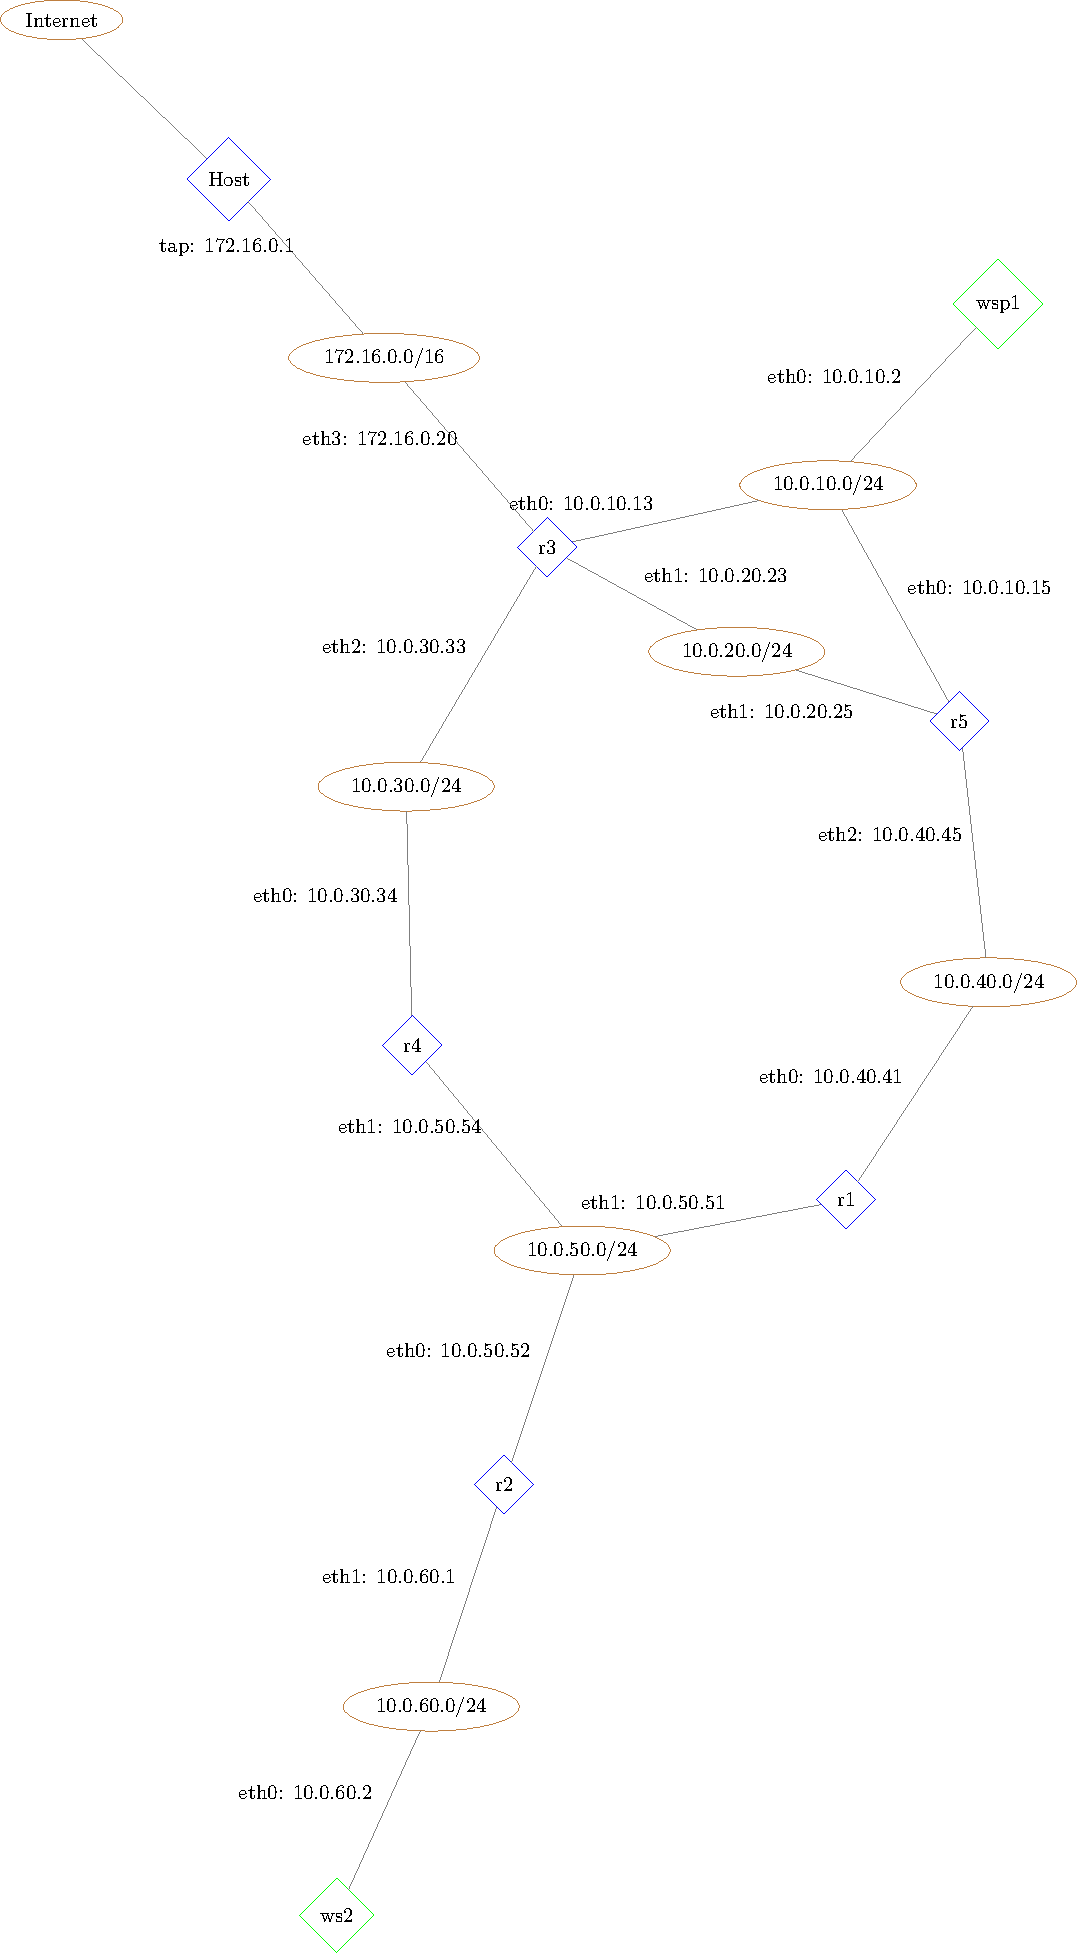
\includegraphics[width=0.8\textwidth]{includes/network_gv.pdf}
\caption{Топология сети}
\label{fig:network}
\end{figure}


Перечень узлов, на которых используется динамическая IP-маршрутизация: 
\begin{itemize}
  \item \textbf{r1-5},
  \item \textbf{wsp1}
\end{itemize}

\clearpage

\section{Назначение IP-адресов}
\begin{itemize}
\item Ниже приведён файл настройки протокола IP маршрутизатора \textbf{r1}.
\inputmintedbr{text}{../../net/r1/etc/network/interfaces}
\item Ниже приведён файл настройки протокола IP маршрутизатора \textbf{r2}.
\inputmintedbr{text}{../../net/r2/etc/network/interfaces}
\item Ниже приведён файл настройки протокола IP маршрутизатора \textbf{r3}.
\inputmintedbr{text}{../../net/r3/etc/network/interfaces}
\item Ниже приведён файл настройки протокола IP маршрутизатора \textbf{r4}.
\inputmintedbr{text}{../../net/r4/etc/network/interfaces}
\item Ниже приведён файл настройки протокола IP маршрутизатора \textbf{r5}.
\inputmintedbr{text}{../../net/r5/etc/network/interfaces}

\item Ниже приведён файл настройки протокола IP рабочей станции \textbf{ws2}.
\inputmintedbr{text}{../../net/ws2/etc/network/interfaces}
\item Ниже приведён файл настройки протокола IP рабочей станции \textbf{wsp1}.
\inputmintedbr{text}{../../net/wsp1/etc/network/interfaces}
\end{itemize}



\subsection{Настройка протокола RIP}
\begin{itemize}
\item Ниже приведен файл \Code{/etc/quagga/ripd.conf} маршрутизатора \textbf{r1}.
\inputmintedbr{text}{../../net/r1/etc/quagga/ripd.conf}
\item Ниже приведен файл \Code{/etc/quagga/ripd.conf} маршрутизатора \textbf{r2}.
\inputmintedbr{text}{../../net/r2/etc/quagga/ripd.conf}
\item Ниже приведен файл \Code{/etc/quagga/ripd.conf} маршрутизатора \textbf{r3}.
\inputmintedbr{text}{../../net/r3/etc/quagga/ripd.conf}
\item Ниже приведен файл \Code{/etc/quagga/ripd.conf} маршрутизатора \textbf{r4}.
\inputmintedbr{text}{../../net/r4/etc/quagga/ripd.conf}
\item Ниже приведен файл \Code{/etc/quagga/ripd.conf} маршрутизатора \textbf{r5}.
\inputmintedbr{text}{../../net/r5/etc/quagga/ripd.conf}
\end{itemize}


Ниже приведен файл \Code{/etc/quagga/ripd.conf} рабочий станции, связанной с несколькими маршрутизаторами \textbf{wsp1}.
\inputmintedbr{text}{../../net/r5/etc/network/interfaces}



\section{Проверка настройки протокола RIP}
Вывод \textbf{traceroute} от \textbf{wsp1} до \textbf{ws2} при нормальной работе сети.
\inputmintedbr{text}{../../results/wsp1-ws2.trace}


Вывод \textbf{traceroute} от узла \textbf{wsp1} до внешнего IP \textbf{8.8.8.8}
\inputmintedbr{text}{../../results/wsp1-world.trace}


Модифицированный udp-клиент для перехвата RIP-сообщений:
\inputmintedbr{c}{../../net/r5/root/ripcatch/ripcatch.c}


Перехваченный обмен сообщениями:
\inputmintedbr{text}{../../results/r5.rip.log}


Таблица RIP:
\inputmintedbr{text}{../../results/r5.vtysh}


Таблица маршрутизации:
\inputmintedbr{text}{../../results/r5.rt}



\section{Расщепленный горизонт и испорченные обратные обновления}
Расщепленный горизонт + испорченные обратные обновления
\inputmintedbr{text}{../../results/r5.sh.pr}


Расщепленный горизонт - испорченные обратные обновления
\inputmintedbr{text}{../../results/r5.sh}


Расщепленный горизонт отключен
\inputmintedbr{text}{../../results/r5.pr}



\section{Имитация устранимой поломки в сети}
Отключаем \textbf{r5}


Вывод таблицы RIP непосредственно перед истечением таймера устаревания (на маршрутизаторе \textbf{r1}).
\inputmintedbr{text}{../../results/r1.r5.route}


Перестроенная таблица на этом же маршрутизаторе
\inputmintedbr{text}{../../results/r1.no-r5.route}


Вывод \textbf{traceroute} от \textbf{ws1} до \textbf{r1} до отключения \textbf{r5}
\inputmintedbr{text}{../../results/wsp1-r1.r5.trace}


Вывод \textbf{traceroute} от \textbf{ws1} до \textbf{r1} после отключения \textbf{r5}
\inputmintedbr{text}{../../results/wsp1-r1.no-r5.trace}



\section{Имитация неустранимой поломки в сети}
Отключаем \textbf{r2}


Таблица на маршрутизаторе \textbf{r5}
\inputmintedbr{text}{../../results/r5.r2-down.vtysh}


Перехват RIP-сообщений на маршрутизаторе \textbf{r5}
\inputmintedbr{text}{../../results/r5.r2-down.ripcatch}
\end{document}
